\documentclass[12pt,oneside,a4paper]{book}

%\usepackage[utf8]{inputenc}
%\usepackage[T1]{fontenc}
\usepackage[english]{babel}

\usepackage{amsmath}
\usepackage{amssymb}
\usepackage{amsthm}
\usepackage{graphics}
\usepackage{enumerate}
\usepackage{amscd}
\usepackage{tikz}
\usetikzlibrary{shapes}

%%%% Layout %%%%%%%%%%%%%%%%%
\addtolength{\evensidemargin}{-2cm}
\addtolength{\oddsidemargin}{-2cm}
\setlength{\textwidth}{17cm} 
\setlength{\textheight}{26.5cm} 
\addtolength{\topmargin}{-3cm}
\setlength{\parindent}{0pt}
\pagestyle{plain}

\newcounter{probnum}
\newcounter{solnum}
\setcounter{probnum}{0}
\newcommand{\prob}{\ifnum\value{probnum}>0\newpage\fi\setcounter{solnum}{0}\stepcounter{probnum}\textbf{Problem \theprobnum}\\}
\newcommand{\ans}{\medskip\hrule\medbreak\emph{Answer: }}
\newcommand{\comment}{\medskip\hrule\medbreak\emph{Comment: }}
\newcommand{\sol}{\medskip\hrule\medbreak\textbf{Solution}\\}
\newcommand{\soln}{\stepcounter{solnum}\medskip\hrule\medbreak\textbf{Solution \thesolnum}\\}
\newcommand{\marking}{\medskip\hrule\medbreak\textbf{Marking scheme -- Problem \theprobnum}}

\newcommand*\circled[1]{\tikz[baseline=(char.base)]{
            \node[shape=circle,draw,inner sep=2pt] (char) {#1};}}

\newcommand{\s}{\phantom{s}}

\begin{document}
\begin{center}
\textbf{\large APMO 1989 -- Problems and Solutions}
\end{center}

% Problem 1
\prob Let $x_1,x_2,\ldots,x_n$ be positive real numbers, and let
\[S=x_1+x_2+\cdots+x_n.\]
Prove that
\[(1+x_1)(1+x_2)\cdots(1+x_n)\le 1 + S + \frac{S^2}{2!} + \frac{S^3}{3!} + \cdots + \frac{S^n}{n!}.\]

\soln
Let $\sigma_k$ be the \emph{$k$th symmetric polynomial}, namely
\[\sigma_k = \sum_{\substack{|S|=k\\ S\subseteq\{1,2,\ldots,n\}}}\prod_{i\in S}x_i,\]
and more explicitly
\[\sigma_1 = S,\quad \sigma_2 = x_1x_2 + x_1x_3 + \cdots + x_{n-1}x_n,\quad \text{and so on.}\]

Then
\[(1+x_1)(1+x_2)\cdots(1+x_n) = 1 + \sigma_1 + \sigma_2 + \cdots + \sigma_n.\]

The expansion of
\[S^k = (x_1+x_2+\cdots+x_n)^k = \underbrace{(x_1+x_2+\cdots+x_n)(x_1+x_2+\cdots+x_n)\cdots (x_1+x_2+\cdots+x_n)}_{k\text{ times}}\]
has at least $k!$ occurrences of $\prod_{i\in S}x_i$ for each subset $S$ with $k$ indices from $\{1,2,\ldots,n\}$. In fact, if $\pi$ is a permutation of $S$, we can choose each $x_{\pi(i)}$ from the $i$th factor of $(x_1+x_2+\cdots+x_n)^k$. Then each term appears at least $k!$ times, and
\[S^k \ge k!\sigma_k\iff \sigma_k \le \frac{S^k}{k!}.\]

Summing the obtained inequalities for $k=1,2,\ldots,n$ yields the result.

\soln
By AM-GM,
\[(1+x_1)(1+x_2)\cdots(1+x_n) \le \left(\frac{(1+x_1)+(1+x_2)+\cdots+(1+x_n)}n\right)^n = \left(1+\frac Sn\right)^n.\]

By the binomial theorem,
\[\left(1+\frac Sn\right)^n = \sum_{k=0}^n\binom nk\left(\frac Sn\right)^k = \sum_{k=0}^n \frac1{k!}\frac{n(n-1)\ldots(n-k+1)}{n^k}S^k \le \sum_{k=0}^n\frac{S^k}{k!},\]
and the result follows.

\comment
\emph{Maclaurin's inequality} states that
\[\frac{\sigma_1}n \ge \sqrt{\frac{\sigma_2}{\binom n2}} \ge \cdots \ge \sqrt[k]{\frac{\sigma_k}{\binom nk}} \ge \cdots \ge \sqrt[n]{\frac{\sigma_n}{\binom nn}}.\]

Then $\sigma_k \le \binom nk\frac{S^k}{n^k} = \frac1{k!}\frac{n(n-1)\ldots(n-k+1)}{n^k}S^k \le \frac{S^k}{k!}$.

% Problem 2
\prob Prove that the equation
\[6(6a^2+3b^2+c^2)=5n^2\]
has no solutions in integers except $a=b=c=n=0$.

\sol
We can suppose without loss of generality that $a,b,c,n\ge 0$. Let $(a,b,c,n)$ be a solution with minimum sum $a+b+c+n$. Suppose, for the sake of contradiction, that $a+b+c+n > 0$.

Since $6$ divides $5n^2$, $n$ is a multiple of $6$. Let $n = 6n_0$. Then the equation reduces to
\[6a^2 + 3b^2 + c^2 = 30n_0^2.\]

The number $c$ is a multiple of $3$, so let $c = 3c_0$. The equation now reduces to
\[2a^2 + b^2 + 3c_0^2 = 10n_0^2.\]

Now look at the equation modulo $8$:
\[b^2 + 3c_0^2 \equiv 2(n_0^2-a^2)\pmod 8.\]

Integers $b$ and $c_0$ have the same parity. Either way, since $x^2$ is congruent to $0$ or $1$ modulo $4$, $b^2 + 3c_0^2$ is a multiple of $4$, so $n_0^2 - a^2 = (n_0-a)(n_0+a)$ is even, and therefore also a multiple of $4$, since $n_0-a$ and $n_0+a$ have the same parity. Hence $2(n_0^2-a^2)$ is a multiple of $8$, and
\[b^2 + 3c_0^2 \equiv 0\pmod 8.\]

If $b$ and $c_0$ are both odd, $b^2+3c_0^2 \equiv 4\pmod 8$, which is impossible. Then $b$ and $c_0$ are both even. Let $b=2b_0$ and $c_0=2c_1$, and we find
\[a^2 + 2b_0^2 + 6c_1^2 = 5n_0^2.\]

Look at the last equation modulo $8$:
\[a^2 + 3n_0^2 \equiv 2(c_1^2 - b_0^2)\pmod 8.\]

A similar argument shows that $a$ and $n_0$ are both even.

We have proven that $a,b,c,n$ are all even. Then, dividing the original equation by $4$ we find
\[6(6(a/2)^2 + 3(b/2)^2 + (c/2)^2) = 5(n/2)^2,\]
and we find that $(a/2,b/2,c/2,n/2)$ is a new solution with smaller sum. This is a contradiction, and the only solution is $(a,b,c,n) = (0,0,0,0)$.

% Problem 3
\prob Let $A_1, A_2, A_3$ be three points in the plane, and for convenience,let $A_4=A_1$, $A_5=A_2$. For $n=1,2,$ and $3$, suppose that $B_n$ is the midpoint of $A_nA_{n+1}$, and suppose that $C_n$ is the midpoint of $A_nB_n$. Suppose that $A_nC_{n+1}$ and $B_nA_{n+2}$ meet at $D_n$, and that $A_nB_{n+1}$ and $C_nA_{n+2}$ meet at $E_n$. Calculate the ratio of the area of triangle $D_1D_2D_3$ to the area of triangle $E_1E_2E_3$.

\ans $\dfrac{25}{49}$.

\sol
Let $G$ be the centroid of triangle $ABC$, and also the intersection point of $A_1B_2$, $A_2B_3$, and $A_3B_1$.

\begin{center}
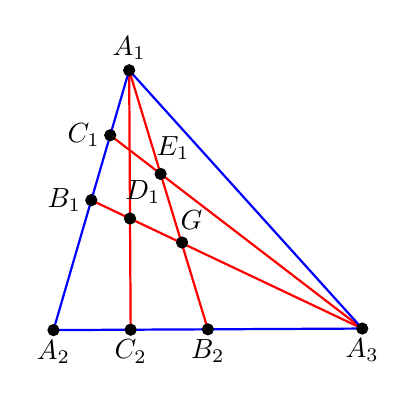
\begin{tikzpicture}
\draw [thick,color=red] (-0.56,4.72)-- (-0.5407903952713049,1.425310578980346) node[anchor=north,color=black] {$C_2$};
\draw [thick,color=red] (-1.04052693018087,3.070207052653564) node[anchor=east,color=black] {$B_1$} -- (2.4,1.44);
\draw [thick,color=red] (0.43947306981913004,1.430207052653564) node[anchor=north,color=black] {$B_2$} -- (-0.56,4.72);
\draw [thick,color=red] (2.4,1.44)-- (-0.800263465090435,3.895103526326782) node[anchor=east,color=black] {$C_1$};
\draw [thick,color=blue] (-0.56,4.72) node[anchor=south,color=black] {$A_1$} -- (2.4,1.44) node[anchor=north,color=black] {$A_3$} -- (-1.5210538603617398,1.4204141053071282) node[anchor=north,color=black] {$A_2$} -- cycle;
\draw [fill=black] (-0.56,4.72) circle (2.pt);
\draw [fill=black] (-1.5210538603617398,1.4204141053071282) circle (2.pt);
\draw [fill=black] (2.4,1.44) circle (2.pt);
\draw [fill=black] (-1.04052693018087,3.070207052653564) circle (2.0pt);
\draw [fill=black] (0.43947306981913004,1.430207052653564) circle (2.0pt);
\draw [fill=black] (-0.800263465090435,3.895103526326782) circle (2.0pt);
\draw [fill=black] (-0.5407903952713049,1.425310578980346) circle (2.0pt);
\draw [fill=black] (-0.5490230830121743,2.837320330845912) circle (2.0pt);
\draw[color=black] (-0.38435485554238596,3.173186616555292) node {$D_1$};
\draw [fill=black] (-0.16021077207234813,3.4040828210614253) circle (2.0pt);
\draw[color=black] (-0.0025628233893205676,3.728520481505205) node {$E_1$};
\draw [fill=black] (0.11210010763931504,2.5325894295289375) circle (2.0pt);
\draw[color=black] (0.2317186508864241,2.817425859321754) node {$G$};
\end{tikzpicture}
\end{center}

By Menelao's theorem on triangle $B_1A_2A_3$ and line $A_1D_1C_2$,
\[\frac{A_1B_1}{A_1A_2}\cdot\frac{D_1A_3}{D_1B_1}\cdot\frac{C_2A_2}{C_2A_3} = 1
\iff \frac{D_1A_3}{D_1B_1} = 2\cdot 3 = 6\iff \frac{D_1B_1}{A_3B_1} = \frac17.\]

Since $A_3G = \frac23A_3B_1$, if $A_3B_1 = 21t$ then $GA_3 = 14t$, $D_1B_1 = \frac{21t}7 = 3t$, $A_3D_1 = 18t$, and $GD_1 = A_3D_1 - A_3G = 18t-14t=4t$, and
\[\frac{GD_1}{GA_3} = \frac4{14} = \frac27.\]

Similar results hold for the other medians, therefore $D_1D_2D_3$ and $A_1A_2A_3$ are homothetic with center $G$ and ratio $-\frac27$.

By Menelao's theorem on triangle $A_1A_2B_2$ and line $C_1E_1A_3$,
\[\frac{C_1A_1}{C_1A_2}\cdot\frac{E_1B_2}{E_1A_1}\cdot\frac{A_3A_2}{A_3B_2} = 1
\iff \frac{E_1B_2}{E_1A_1} = 3\cdot \frac12 = \frac32\iff \frac{A_1E_1}{A_1B_2} = \frac25.\]

If $A_1B_2 = 15u$, then $A_1G = \frac23\cdot 15u = 10u$ and $GE_1 = A_1G - A_1E_1 = 10u - \frac25\cdot 15u = 4u$, and
\[\frac{GE_1}{GA_1} = \frac 4{10} = \frac25.\]

Similar results hold for the other medians, therefore $E_1E_2E_3$ and $A_1A_2A_3$ are homothetic with center $G$ and ratio $\frac25$.

Then $D_1D_2D_3$ and $E_1E_2E_3$ are homothetic with center $G$ and ratio $-\frac 27 : \frac25 = -\frac57$, and the ratio of their area is $\left(\frac 57\right)^2 = \frac{25}{49}$.

% Problem 4
\prob Let $S$ be a set consisting of $m$ pairs $(a,b)$ of positive integers with the property that $1\le a<b\le n$. Show that there are at least
\[4m\frac{(m-\frac{n^2}4)}{3n}\]
triples $(a,b,c)$ such that $(a,b)$, $(a,c)$, and $(b,c)$ belong to $S$.

\sol
Call a triple $(a,b,c)$ \emph{good} if and only if $(a,b)$, $(a,c)$, and $(b,c)$ all belong to $S$. For $i$ in $\{1,2,\ldots,n\}$, let $d_i$ be the number of pairs in $S$ that contain $i$, and let $D_i$ be the set of numbers paired with $i$ in $S$ (so $|D_i| = d_i$). Consider a pair $(i,j)\in S$. Our goal is to estimate the number of integers $k$ such that any permutation of $\{i,j,k\}$ is good, that is, $|D_i\cap D_j|$. Note that $i\notin D_i$ and $j\notin D_j$, so $i,j\notin D_i\cap D_j$; thus any $k\in D_i\cap D_j$ is different from both $i$ and $j$, and $\{i,j,k\}$ has three elements as required. Now, since $D_i\cup D_j \in \{1,2,\ldots,n\}$,
\[|D_i\cap D_j| = |D_i| + |D_j| - |D_i\cup D_j| \le d_i + d_j - n.\]

Summing all the results, and having in mind that each good triple is counted three times (one for each two of the three numbers), the number of good triples $T$ is at least
\[T \ge \frac 13\sum_{(i,j)\in S}(d_i+d_j-n).\]

Each term $d_i$ appears each time $i$ is in a pair from $S$, that is, $d_i$ times; there are $m$ pairs in $S$, so $n$ is subtracted $m$ times. By the Cauchy-Schwartz inequality
\[T \ge \frac13\left(\sum_{i=1}^n d_i^2 - mn\right) \ge \frac13\left(\frac{\left(\sum_{i=1}^n d_i\right)^2}n - mn\right).\]

Finally, the sum $\sum_{i=1}^n d_i$ is $2m$, since $d_i$ counts the number of pairs containing $i$, and each pair $(i,j)$ is counted twice: once in $d_i$ and once in $d_j$. Therefore
\[T \ge \frac13\left(\frac{(2m)^2}n - mn\right) = 4m\frac{(m-\frac{n^2}4)}{3n}.\]

\comment
This is a celebrated graph theory fact named \emph{Goodman's bound}, after A.~M.~Goodman's method published in 1959. The generalized version of the problem is still studied until today.

% Problem 5
\prob Determine all functions $f$ from the reals to the reals for which
\begin{enumerate}[(1)]
\item $f(x)$ is strictly increasing,
\item $f(x)+g(x)=2x$ for all real $x$,
where $g(x)$ is the composition inverse function to $f(x)$.
\end{enumerate}
(\emph{Note}: $f$ and $g$ are said to be composition inverses if $f(g(x))=x$ and $g(f(x))=x$ for all real $x$.)

\ans $f(x) = x+c$, $c\in\mathbb{R}$ constant.

\sol
Denote by $f_n$ the $n$th iterate of $f$, that is, $f_n(x) = \underbrace{f(f(\ldots f}_{n\text{ times}}(x)))$.

Plug $x\to f_{n+1}(x)$ in (2): since $g(f_{n+1}(x)) = g(f(f_n(x))) = f_n(x)$,
\[f_{n+2}(x) + f_n(x) = 2f_{n+1}(x),\]
that is,
\[f_{n+2}(x) - f_{n+1}(x) = f_{n+1}(x) - f_n(x).\]

Therefore $f_n(x) - f_{n-1}(x)$ does not depend on $n$, and is equal to $f(x)-x$. Summing the corresponding results for smaller values of $n$ we find
\[f_n(x) - x = n(f(x)-x).\]

Since $g$ has the same properties as $f$,
\[g_n(x) - x = n(g(x)-x) = -n(f(x)-x).\]

Finally, $g$ is also increasing, because since $f$ is increasing $g(x) > g(y)\implies f(g(x)) > f(g(y)) \implies x > y$. An induction proves that $f_n$ and $g_n$ are also increasing functions.

Let $x>y$ be real numbers. Since $f_n$ and $g_n$ are increasing,
\[x + n(f(x)-x) > y + n(f(y)-y)\iff n[(f(x)-x) - (f(y)-y)] > y-x\]
and
\[x - n(f(x)-x) > y - n(f(y)-y)\iff n[(f(x)-x) - (f(y)-y)] < x-y.\]

Summing it up,
\[|n[(f(x)-x) - (f(y)-y)]| < x-y\quad\text{for all }n\in\mathbb{Z}_{>0}.\]

Suppose that $a = f(x)-x$ and $b = f(y)-y$ are distinct. Then, for all positive integers $n$,
\[|n(a-b)| < x-y,\]
which is false for a sufficiently large $n$. Hence $a=b$, and $f(x)-x$ is a constant $c$ for all $x\in\mathbb{R}$, that is, $f(x) = x+c$.

It is immediate that $f(x)=x+c$ satisfies the problem, as $g(x) = x-c$.
\end{document}